% !TEX program = xelatex
\documentclass{misisarticle}
\usepackage{float}
\usepackage{placeins}
\usepackage{balance}

\grnti{}
\asjc{}
\oecd{}

\title{Применение искусственного интеллекта для обнаружения дефектов на промышленных изображениях}

\misisauthor{Н.Е. Орлов}{кафедра инженерной кибернетики НИТУ «МИСиС»}{Москва, Россия}{m241061@edu.missis.ru}

\setabstract{Автоматическое обнаружение дефектов металлических поверхностей является важной задачей промышленного визуального контроля, требующей точной локализации при ограниченных вычислительных затратах. Цель работы~--- сравнить YOLOv8n и YOLO11n и оценить влияние умеренных аугментаций на обнаружение дефектов стальной поверхности. Исследование выполнено на подготовленном наборе NEU-DET из 1799 изображений и 4183 аннотированных объектов шести классов. Рассмотрены четыре конфигурации детекторов с аугментациями и без них при одинаковых основных параметрах обучения. Качество оценивалось по Precision, Recall, F1, mAP@50 и mAP@50:95; дополнительно проведены анализ ошибок и измерение задержки. Применение аугментаций сопровождалось увеличением mAP@50:95 на 9,33 процентного пункта для YOLOv8n и на 9,27 для YOLO11n. Наилучший результат получен для YOLOv8n с аугментациями: mAP@50:95 составила 37,29\%, фиксированная F1~--- 67,25\%, а средняя задержка обработки~--- 7,98~мс. Обобщение результатов требует повторных экспериментов и проверки на независимых промышленных изображениях.}
\setkeywords{компьютерное зрение, обнаружение дефектов, глубокое обучение, YOLOv8, YOLO11, NEU-DET, аугментация данных}

\begin{document}
\maketitle

\section{Введение}
Обеспечение качества металлических изделий относится к важным задачам промышленного производства. Поверхностные дефекты, возникающие при изготовлении и обработке стального проката, могут ухудшать эксплуатационные характеристики продукции и приводить к дополнительным затратам. Для их своевременного выявления необходим визуальный контроль, способный различать нарушения неодинаковых формы, масштаба и контраста~\cite{ibrahim2024}.

При ручной инспекции результат зависит от человеческого фактора, а традиционные методы, опирающиеся на яркостные, текстурные и геометрические признаки, могут быть чувствительны к неоднородности поверхности и изменениям условий съёмки~\cite{ibrahim2024,chazhoor2024}. Нейросетевые детекторы позволяют автоматически извлекать признаки и определять не только тип дефекта, но и его положение на изображении.

Одностадийные модели семейства YOLO (\textit{You Only Look Once}) выполняют предсказание классов и ограничивающих прямоугольников в рамках единого вычислительного процесса~\cite{redmon2016}. Компактные реализации YOLOv8n и YOLO11n представляют интерес для задач, в которых наряду с качеством обнаружения учитываются вычислительные затраты~\cite{jocher2023,jocher2024}. В современных исследованиях рассматриваются облегчённые варианты YOLOv8n и модификации YOLO11 с улучшенным извлечением и объединением признаков~\cite{liu2024,ni2025,li2026}. При этом результаты, полученные при различных разделениях данных и протоколах оценки, нельзя непосредственно сравнивать между собой.

В ряде исследований рассматриваются и другие подходы к анализу промышленных дефектов: Гаскаров и соавторы применяли свёрточные сети для сегментации дефектов стальных листов~\cite{gaskarov2020}; Андриянов и соавторы исследовали методы сегментации изображений металлических изделий на основе компьютерного зрения~\cite{andriyanov2023}; Васильев и соавторы рассматривали обнаружение дефектов поверхности изделий с использованием YOLOv5 и его модификации~\cite{vasiliev2024}. Указанные работы иллюстрируют разнообразие постановок задачи; результаты сегментации и детекции нельзя непосредственно сопоставлять по одной метрике.

При ограниченном количестве размеченных изображений одним из доступных приёмов является расширение разнообразия обучающих примеров посредством геометрических и фотометрических аугментаций~\cite{shorten2019}. Однако их эффект необходимо оценивать отдельно для конкретного набора данных и архитектуры. Цель работы~--- экспериментально сравнить YOLOv8n и YOLO11n при обнаружении дефектов поверхности стали на NEU-DET и оценить влияние умеренных аугментаций при фиксированных условиях обучения и тестирования. Для достижения цели проведены четыре эксперимента, исследованы качество детекции, ошибки и задержка обработки изображений.

\section{Материалы и методы}
\begin{figure*}[t]
  \centering
  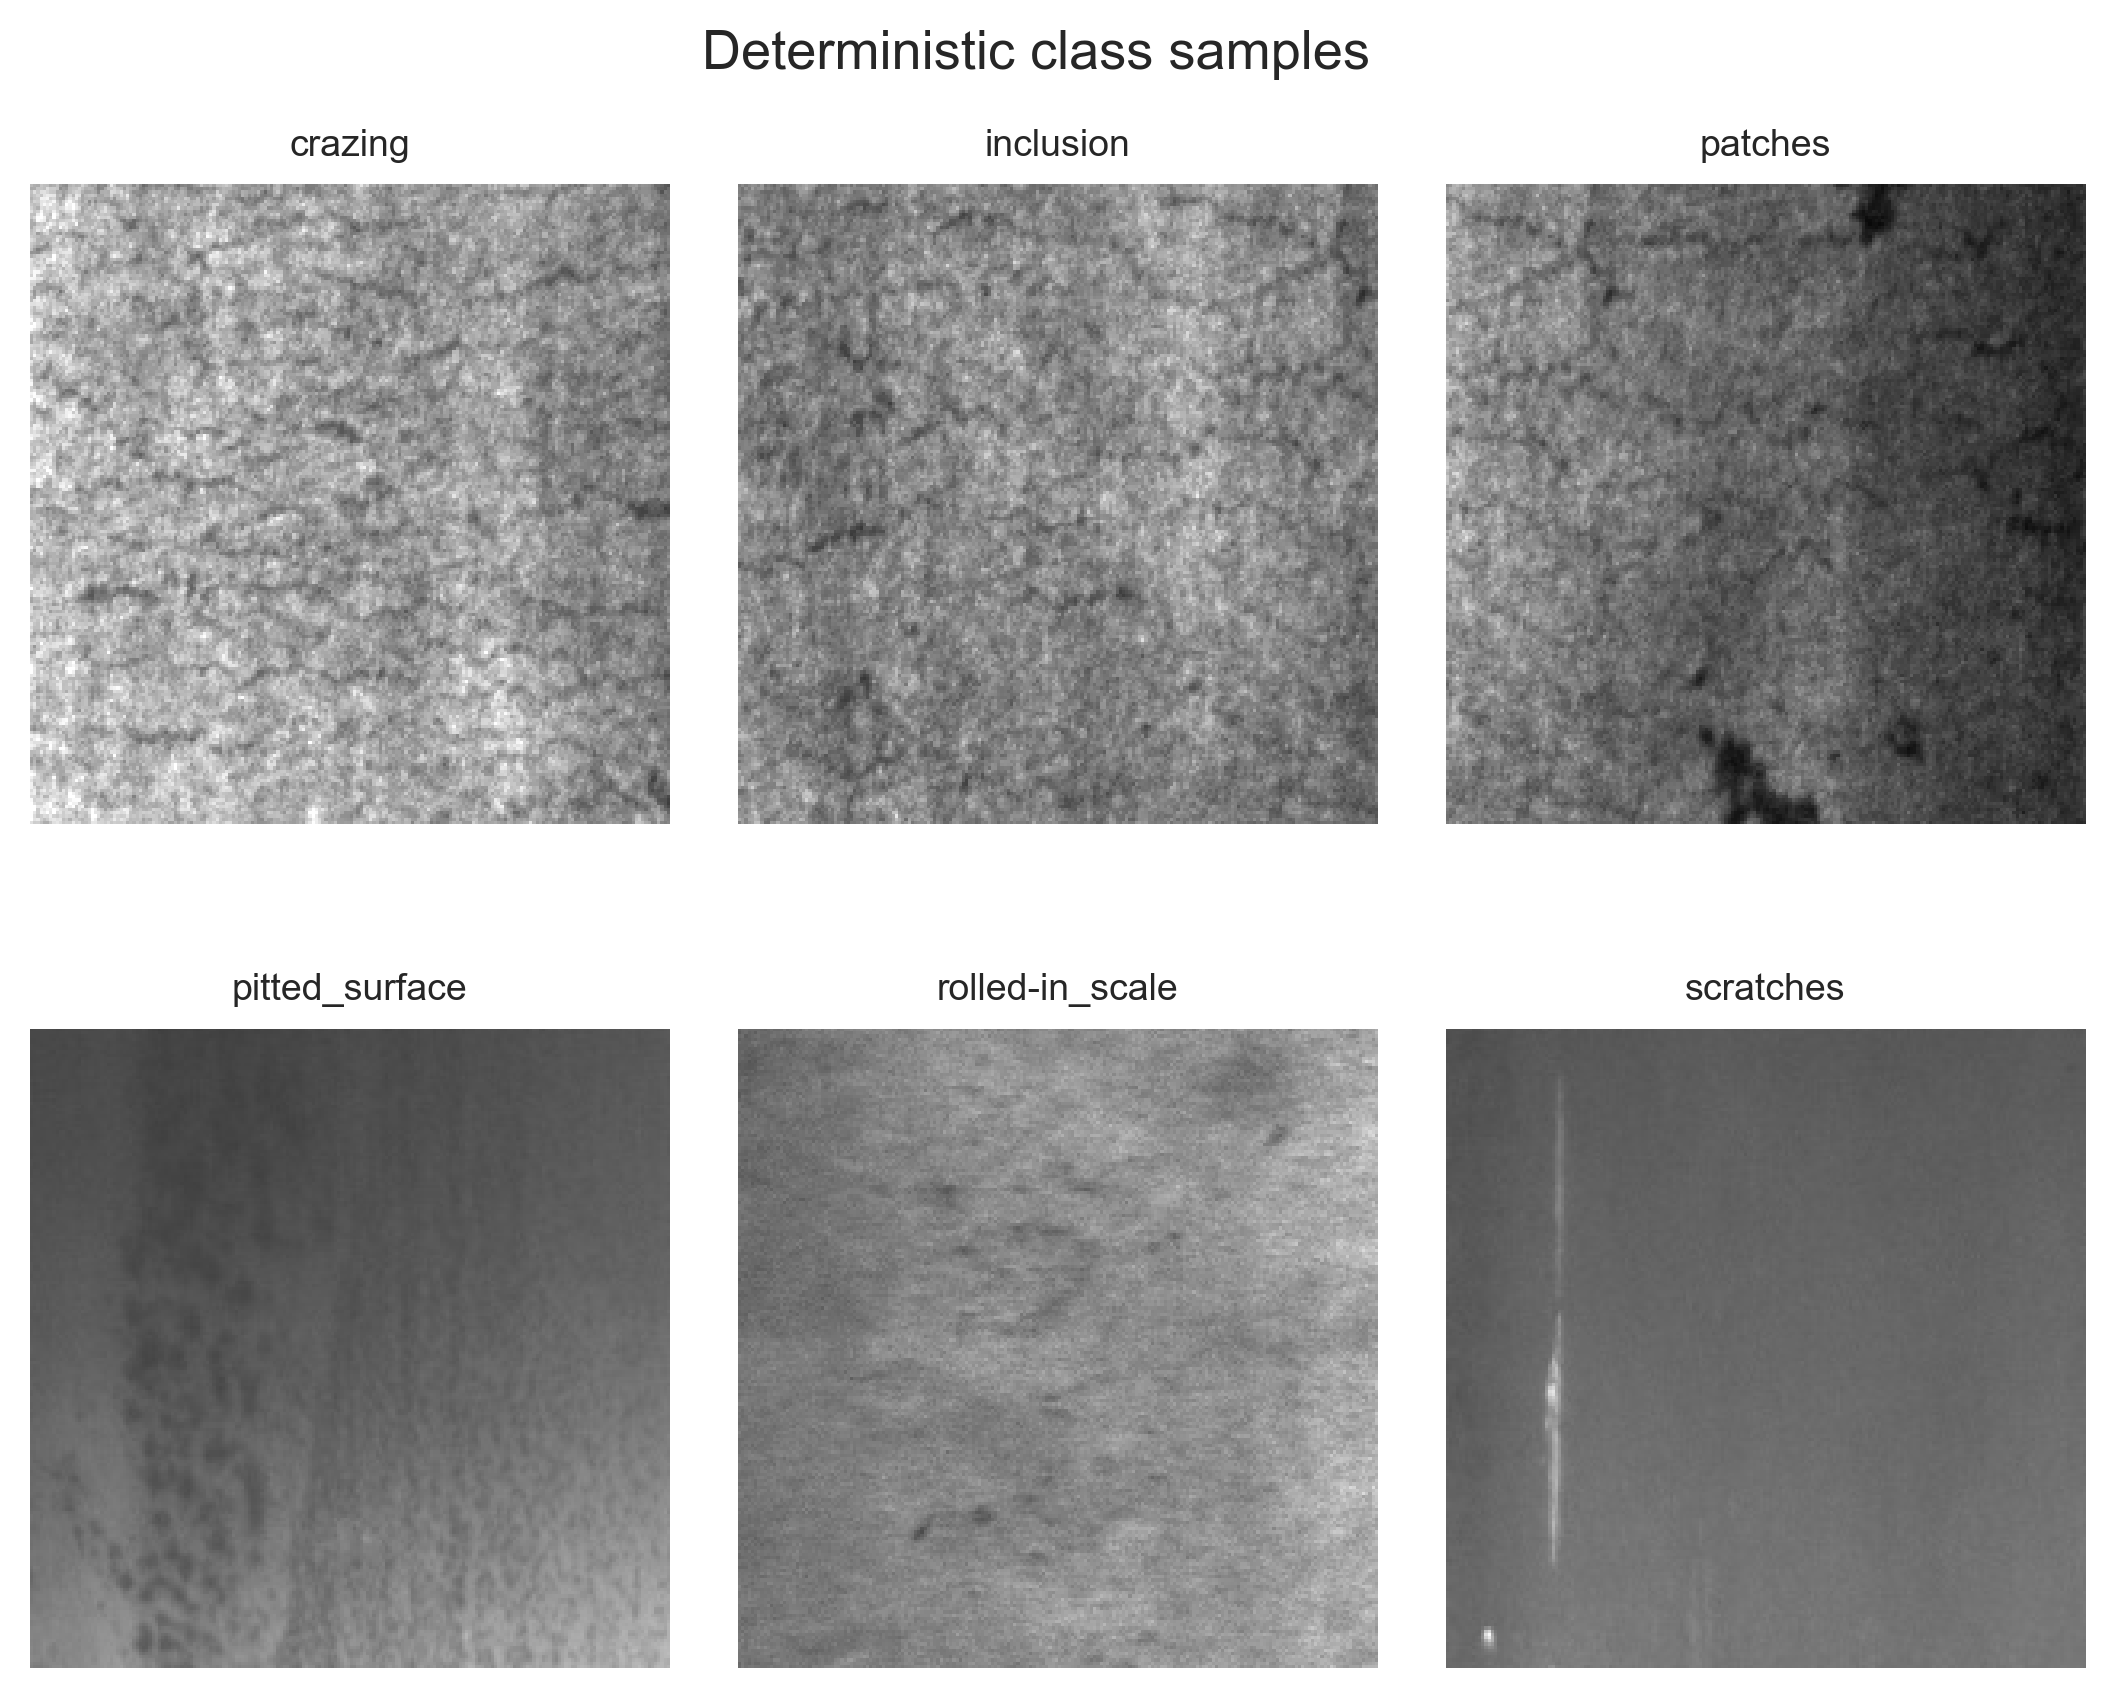
\includegraphics[width=0.73\textwidth]{figures/fig_1_class_samples.png}
  \caption{Примеры изображений шести типов дефектов из NEU-DET.}
  \label{fig:classes}
\end{figure*}

\subsection{Набор данных и подготовка}
Для исследования использован набор NEU-DET (\textit{Northeastern University Surface Defect Detection}), предназначенный для локализации дефектов стальной поверхности. Его основой является база NEU, представленная K.~Song и Y.~Yan~\cite{song2013}; детекционная постановка с координатами ограничивающих прямоугольников описана Y.~He и соавторами~\cite{he2020}. Фактическая версия разметки Pascal VOC получена из открытого репозитория ETDNet\footnote{\url{https://github.com/zht8506/ETDNet}}.

Набор содержит шесть типов дефектов: \textit{crazing} (трещинообразные нарушения), \textit{inclusion} (включения), \textit{patches} (пятна), \textit{pitted surface} (точечные углубления), \textit{rolled-in scale} (вкатанная окалина) и \textit{scratches} (царапины). Исходное разрешение каждого изображения~--- $200\times200$ пикселей. В выбранном каноническом наборе было 1800 изображений и 4189 записей объектов в XML-аннотациях.

При проверке обнаружены два изображения с идентичным содержимым, но различающимися аннотациями; один экземпляр исключён. Удалены также три повторяющиеся записи объектов. Исходные JPEG/XML не изменялись. После очистки осталось 1799 изображений с 4183 объектами. Разбиение на обучающую, валидационную и тестовую части выполнено детерминированно при $\mathrm{seed}=42$ со стратификацией по основному классу изображения; статистика представлена в табл.~\ref{tab:dataset}, а примеры классов~--- на рис.~\ref{fig:classes}. Для многообъектных изображений сохранена полная разметка. Проверка SHA-256 не выявила точных межвыборочных дубликатов. Координаты прямоугольников преобразованы из Pascal VOC в нормализованный формат YOLO.

% Таблица I — собственный, очищенный датасет NEU-DET
\begin{table}[t]
\caption{Распределение изображений и объектов NEU-DET}
\label{tab:dataset}
\centering
\footnotesize
\setlength{\tabcolsep}{3.7pt}
\begin{tabular}{@{}lrr@{}}
\toprule
Выборка & Изображения & Объекты \\
\midrule
Обучающая (Train) & 1223 & 2804 \\
Валидационная (Val) & 216 & 521 \\
Тестовая (Test) & 360 & 858 \\
\midrule
\textbf{Всего} & \textbf{1799} & \textbf{4183} \\
\bottomrule
\end{tabular}
\end{table}


Обучающая выборка использовалась для оптимизации параметров моделей, валидационная~--- для контроля обучения и выбора контрольной точки; тестовая оставалась неизменной до итоговой оценки. Созданное разбиение является протоколом данного исследования, а не официальным разделением NEU-DET.

\subsection{Архитектуры и показатели качества}
Сопоставлялись предобученные модели YOLOv8n и YOLO11n, реализованные в библиотеке Ultralytics~\cite{jocher2023,jocher2024}. Обе относятся к одностадийным детекторам, но имеют различия в архитектуре извлечения и объединения признаков. Выбор вариантов \textit{nano} обусловлен интересом к компромиссу между качеством и вычислительной сложностью: число параметров составляет около 3,01 млн для YOLOv8n и 2,58 млн для YOLO11n.

Для оценки применялись Precision ($P$), Recall ($R$), F1 и средняя точность детекции (mAP). Корректность пересечения предсказанного и эталонного прямоугольников характеризовалась показателем $IoU=|A\cap B|/|A\cup B|$. Основные показатели вычислялись по формулам:
\begin{equation}
 P=\frac{TP}{TP+FP},\quad R=\frac{TP}{TP+FN},\quad F_1=\frac{2PR}{P+R},
\label{eq:prf}
\end{equation}
где $TP$, $FP$ и $FN$ обозначают истинно положительные, ложноположительные и пропущенные обнаружения соответственно. Значение $mAP@50$ представляет среднее по классам AP при $IoU=0{,}50$; $mAP@50{:}95$ усредняет AP по десяти порогам от 0,50 до 0,95 с шагом 0,05, следуя принятому COCO-подобному подходу к оценке~\cite{lin2014}.

Метрики mAP рассчитывались стандартными средствами Ultralytics при пороге уверенности 0,001 и NMS IoU = 0,70. Precision, Recall и F1 вычислялись отдельно при пороге уверенности 0,25, сопоставлении предсказаний с истинными объектами одного класса по убыванию уверенности и условии взаимно однозначного соответствия при IoU $\geq0{,}50$. Для P/R/F1 использовалось микроусреднение по всем классам; таким образом, фиксированные P/R/F1 и mAP относятся к разным протоколам и дополняют друг друга.

\section{Экспериментальное исследование}
Организованы четыре независимых эксперимента с двумя факторами: архитектурой и применением аугментаций. В E1 (YOLOv8n) и E2 (YOLO11n) случайные преобразования обучающих изображений были отключены (\textit{baseline}); в E3 (YOLOv8n) и E4 (YOLO11n) использовался одинаковый профиль умеренных аугментаций (\textit{augmented}). Начальные веса всех моделей были предобучены; перенос оптимизированных весов между четырьмя запусками не выполнялся.

Общими условиями являлись размер входа $320\times320$ пикселей, пакет из 16 изображений, оптимизатор AdamW, начальная скорость обучения $10^{-3}$, весовая регуляризация $5\cdot10^{-4}$, максимум 100 эпох, $\mathrm{seed}=42$, детерминированный режим и автоматическая смешанная точность (AMP). Ранняя остановка активировалась при отсутствии улучшения валидационного критерия на протяжении 20 эпох. Сохранённая контрольная точка \texttt{best.pt} выбиралась по валидационной выборке; для E1--E4 получено соответственно 36, 63, 100 и 95 эпох обучения.

Профиль \textit{augmented} включал горизонтальное и вертикальное отражение с вероятностью 0,5, поворот до $\pm5^\circ$, смещение до 5\% размера изображения, масштабирование в пределах 10\% и изменение яркостного канала V в HSV с параметром 0,10. Преобразования Mosaic, MixUp, CutMix и дополнительные неявные операции Albumentations были отключены. Следовательно, различие внутри каждой пары E1/E3 и E2/E4 определялось заданным набором аугментаций при одинаковых основных параметрах обучения.

Вычисления выполнялись в среде Windows 11, Python 3.12.10, PyTorch 2.7.1+cu128, Ultralytics 8.3.239 на NVIDIA GeForce RTX 4070 Laptop GPU с 8 ГиБ видеопамяти. Финальная оценка всех контрольных точек проведена на отдельной Test-выборке по заранее заданному протоколу; тестовые изображения не использовались для подбора порогов, гиперпараметров или выбора модели.

\section{Результаты и обсуждение}
\subsection{Сравнение моделей и аугментаций}
Итоговые результаты на тестовой выборке приведены в табл.~\ref{tab:test_metrics}. В базовом режиме YOLOv8n (E1) показала $mAP@50{:}95=27{,}96\%$, тогда как YOLO11n (E2)~--- 27,25\%; различие составило 0,71 процентного пункта (п.п.). При этом E2 характеризовалась более высокой Precision (64,32\% против 57,26\%) и меньшей Recall (62,82\% против 71,68\%). Близкие значения фиксированного F1 (63,66 и 63,56\%) скрывают различия в соотношении ложных срабатываний и пропусков.

% Таблица II — итоговая оценка на независимой Test-выборке
\begin{table*}[t]
\caption{Качество обнаружения на Test, \%. P/R/F1: fixed conf=0,25 и IoU=0,50; mAP: стандартный протокол Ultralytics}
\label{tab:test_metrics}
\centering
\small
\begin{tabular*}{0.91\textwidth}{@{\extracolsep{\fill}}lccccc@{}}
\toprule
Модель & Precision & Recall & F1 & mAP@50 & mAP@50:95 \\
\midrule
E1: YOLOv8n, baseline & 57,26 & 71,68 & 63,66 & 59,68 & 27,96 \\
E2: YOLO11n, baseline & 64,32 & 62,82 & 63,56 & 53,61 & 27,25 \\
\textbf{E3: YOLOv8n, augmented} & 60,31 & \textbf{75,99} & \textbf{67,25} & \textbf{72,32} & \textbf{37,29} \\
E4: YOLO11n, augmented & 57,98 & 75,76 & 65,69 & 71,14 & 36,52 \\
\bottomrule
\end{tabular*}
\end{table*}


Использование умеренных аугментаций сопровождалось повышением $mAP@50{:}95$ для обеих архитектур: при переходе E1$\to$E3 прирост составил 9,33 п.п. (27,96$\to$37,29\%), а E2$\to$E4~--- 9,27 п.п. (27,25$\to$36,52\%). Фиксированный F1 увеличился соответственно на 3,59 и 2,13 п.п. Для E3 возросли как Precision, так и Recall; для E4 рост Recall сопровождался снижением Precision относительно E2. Следовательно, улучшение интегральной метрики не означает одновременного роста всех частных показателей.

Наибольшие $mAP@50{:}95$ (37,29\%) и F1 (67,25\%) в данном протоколе получила YOLOv8n с аугментациями (E3). Её преимущество над E4 по $mAP@50{:}95$ составляет около 0,77 п.п. При одном запуске каждой конфигурации это различие не даёт оснований считать одну архитектуру универсально превосходящей другую.

\subsection{Поклассовое качество и характер ошибок}
Поклассовые результаты на рис.~\ref{fig:perclass} демонстрируют неодинаковую сложность обнаружения дефектов. Для E3 AP@50:95 составила 13,88\% для \textit{crazing}, 22,23\% для \textit{rolled-in scale}, 39,87\% для \textit{inclusion}, 46,11\% для \textit{pitted surface}, 46,32\% для \textit{scratches} и 55,30\% для \textit{patches}. Наиболее трудными оставались \textit{crazing} и \textit{rolled-in scale}. Для обеих архитектур использование аугментаций сопровождалось ростом AP@50:95 во всех шести классах, однако неоднородность результатов сохранилась.

\begin{figure*}[t]
  \centering
  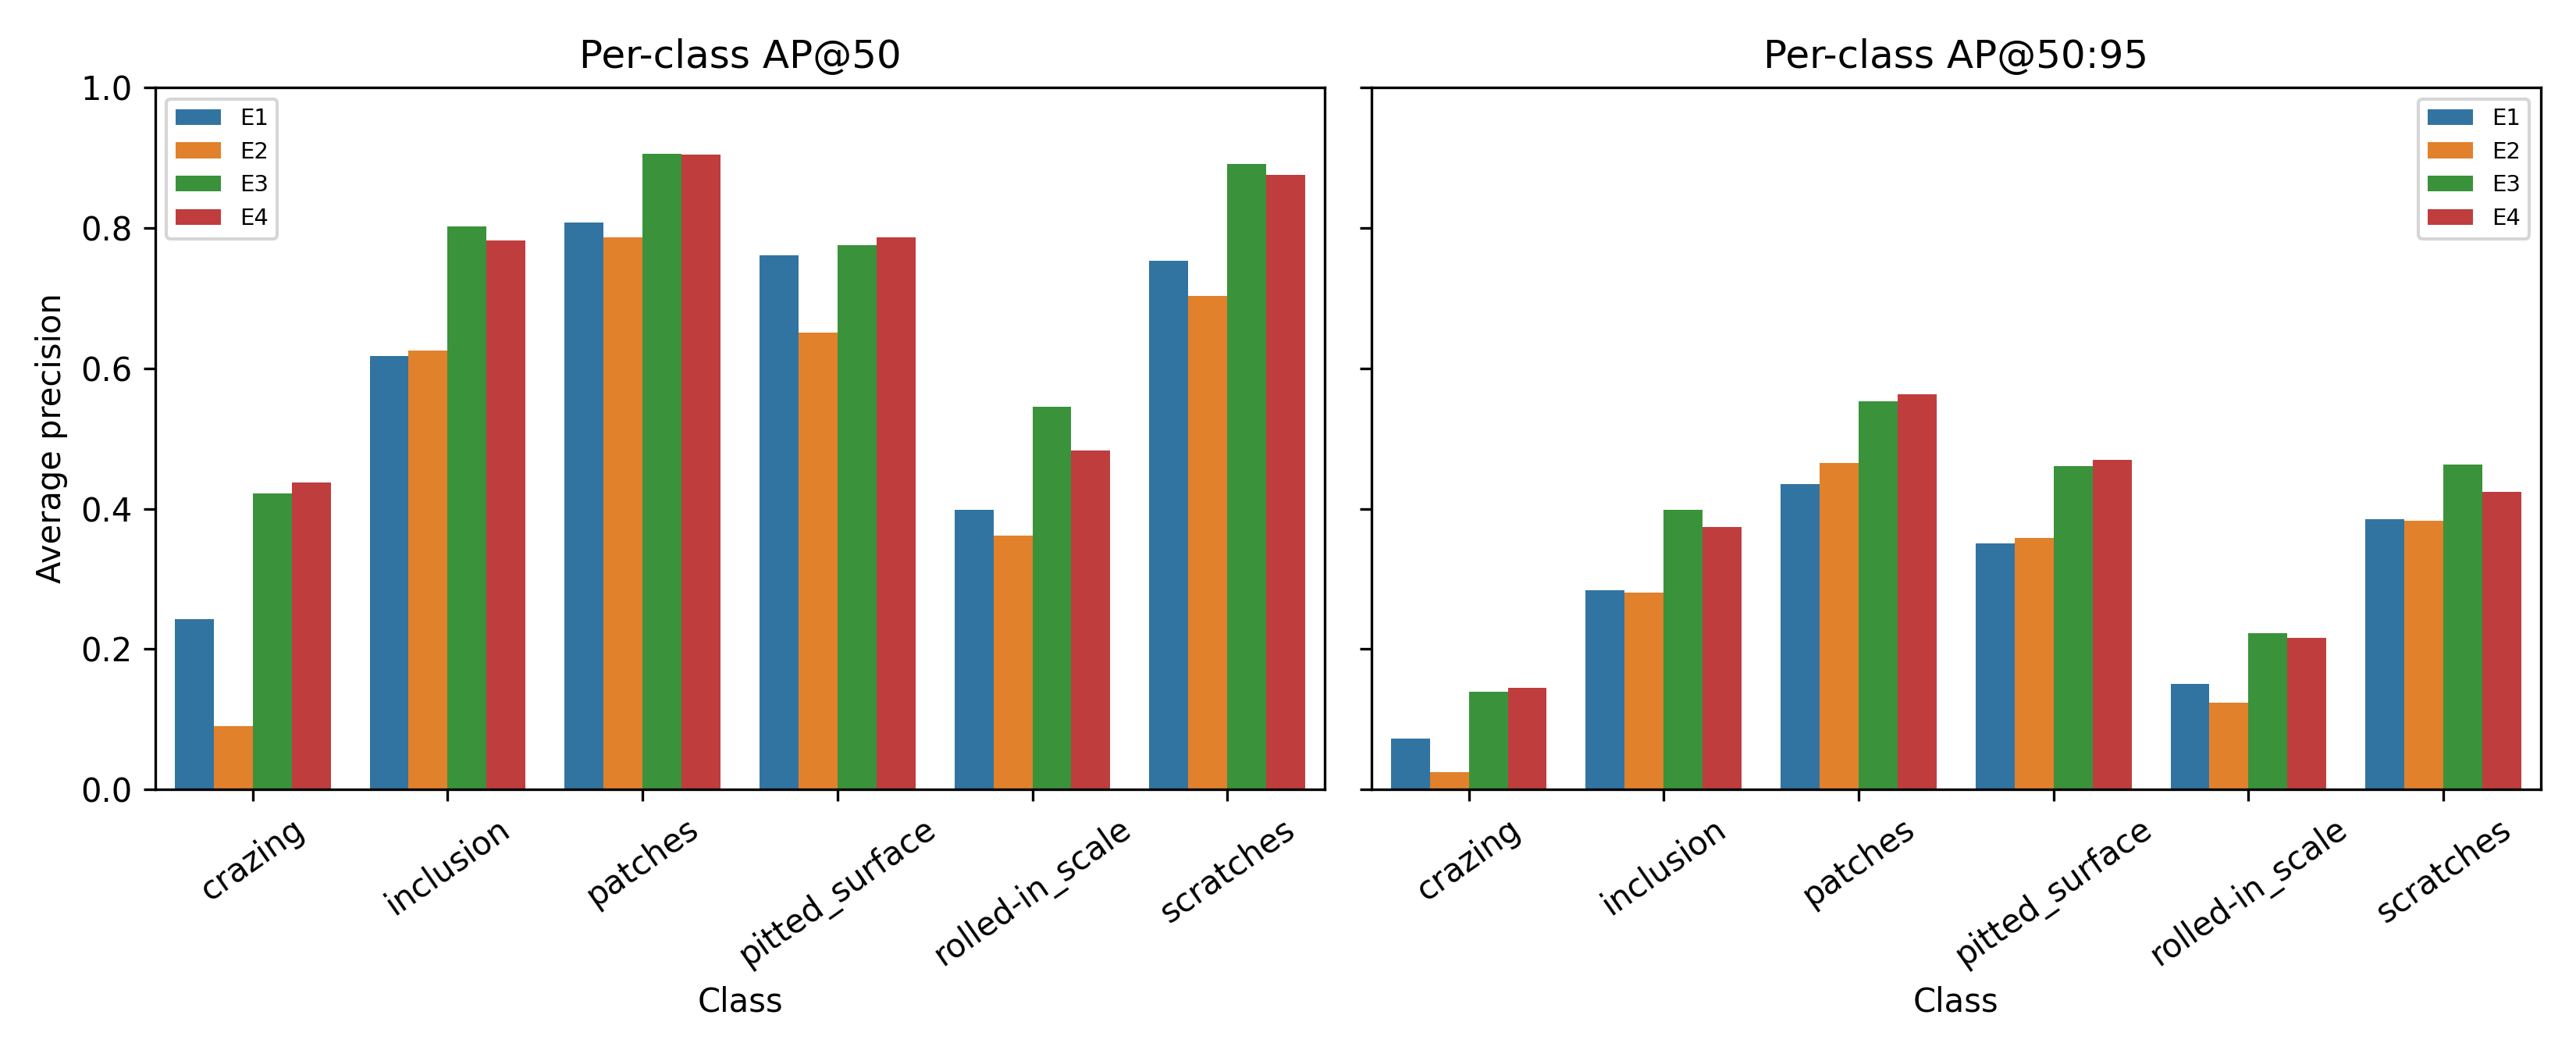
\includegraphics[width=0.92\textwidth]{figures/fig_4_per_class_ap.png}
  \caption{Поклассовые AP@50 (слева) и AP@50:95 (справа) на Test для E1--E4.}
  \label{fig:perclass}
\end{figure*}

Низкое качество на отдельных классах может быть обусловлено невыраженными границами, сложной текстурой и малым размером дефектов. Такие проблемы рассматриваются также в работах по модификации промышленных YOLO-детекторов~\cite{ni2025,li2026}. Однако в настоящем исследовании не выполнялся отдельный причинный анализ этих факторов.

При фиксированном пороге уверенности E3 получила $TP=652$, $FP=429$ и $FN=206$ против $615$, $459$ и $243$ у E1. Основная диагностическая категория FP~--- \texttt{overlap\_fp}: предсказания, имеющие ненулевое IoU с хотя бы одним объектом эталонной разметки независимо от класса. Для E3 зарегистрировано 307 таких предсказаний. Эта категория \emph{не равнозначна} ошибке локализации, поскольку включает любые пространственные пересечения, в том числе малые.

Из 858 объектов Test 102 отнесены к малым по условию площади рамки меньше $1024~\text{пикселей}^2$ на исходном изображении. Число пропусков таких объектов составило 30, 50, 25 и 19 для E1--E4 соответственно. Таким образом, E4 пропустила меньше малых объектов, чем E3, несмотря на более низкий интегральный $mAP@50{:}95$. Пример ошибок на изображении \textit{rolled-in scale} для E3 приведён на рис.~\ref{fig:failure}.

\begin{figure}[t]
  \centering
  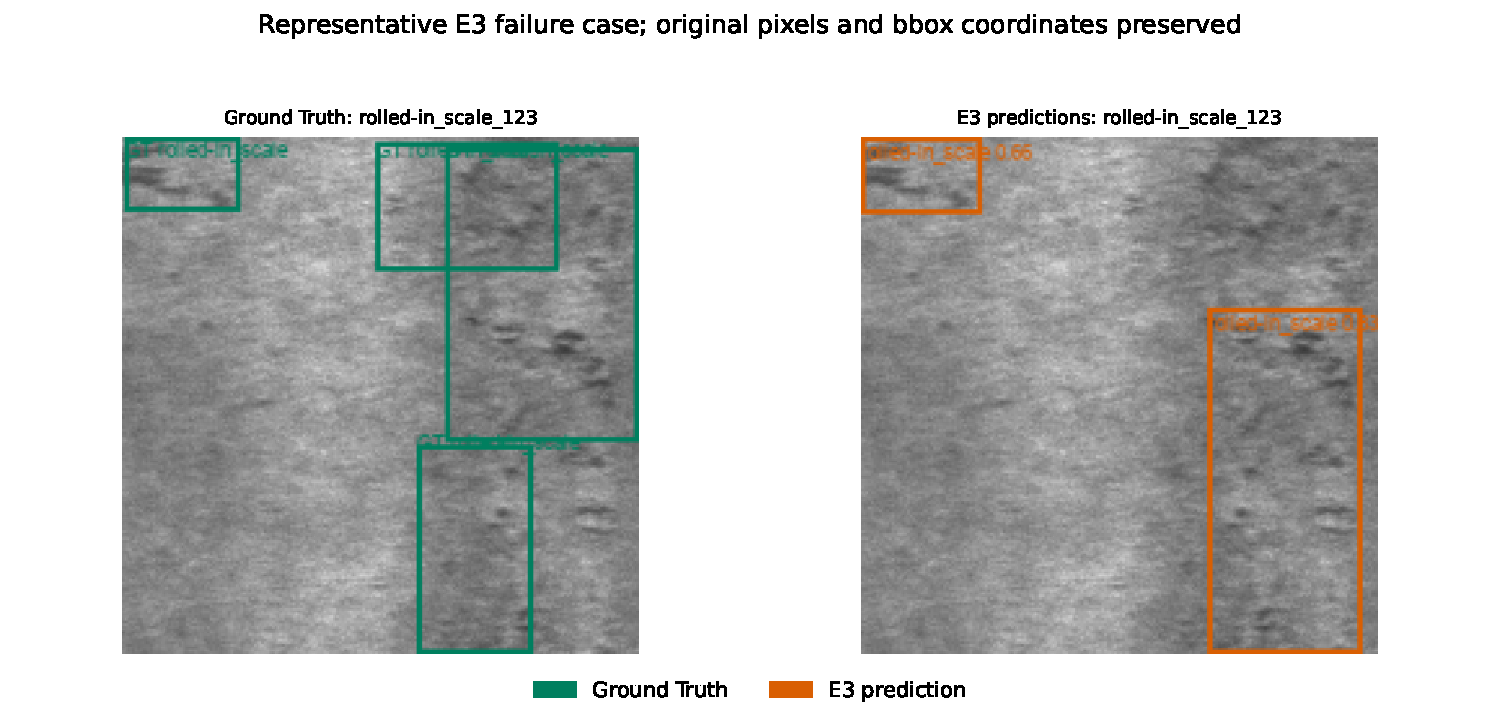
\includegraphics[width=\columnwidth]{figures/fig_6_failure_case.pdf}
  \caption{Пример сравнения эталонной разметки и предсказаний E3 на изображении \textit{rolled-in scale}.}
  \label{fig:failure}
\end{figure}

\subsection{Вычислительная производительность}
Измерения на RTX 4070 Laptop GPU выполнялись при FP32, $320\times320$ пикселей и размере пакета 1. После 30 прогревочных запусков были проведены 100 измерений с синхронизацией CUDA. Задержка \textit{forward} относится только к проходу сети по заранее подготовленному тензору, а \textit{end-to-end} (E2E) дополнительно включает чтение изображения и пред- и постобработку. Результаты приведены в табл.~\ref{tab:latency}.

% Таблица III
\begin{table}[t]
\caption{Измеренная задержка инференса, мс}
\label{tab:latency}
\centering
\footnotesize
\setlength{\tabcolsep}{2.6pt}
\begin{tabular}{@{}lrrrr@{}}
\toprule
Модель & Парам., млн & Forward & E2E & P95 \\
\midrule
E1 & 3,01 & 5,37 & 7,97 & 9,65 \\
E2 & 2,58 & 7,36 & 9,68 & 12,06 \\
E3 & 3,01 & 5,47 & 7,98 & 9,58 \\
E4 & 2,58 & 7,53 & 9,93 & 12,44 \\
\bottomrule
\end{tabular}
\end{table}


Модели E1 и E3 продемонстрировали близкую среднюю задержку E2E~--- 7,97 и 7,98 мс; у E2 и E4 значения выше~--- 9,68 и 9,93 мс. При этом YOLO11n имеет меньше параметров, что подчёркивает ограниченность числа параметров как единственного показателя скорости. Сопоставление качества и задержки (рис.~\ref{fig:tradeoff}) показывает, что E3 обеспечивает наибольший $mAP@50{:}95$ при задержке, практически не отличающейся от E1.

\begin{figure}[t]
  \centering
  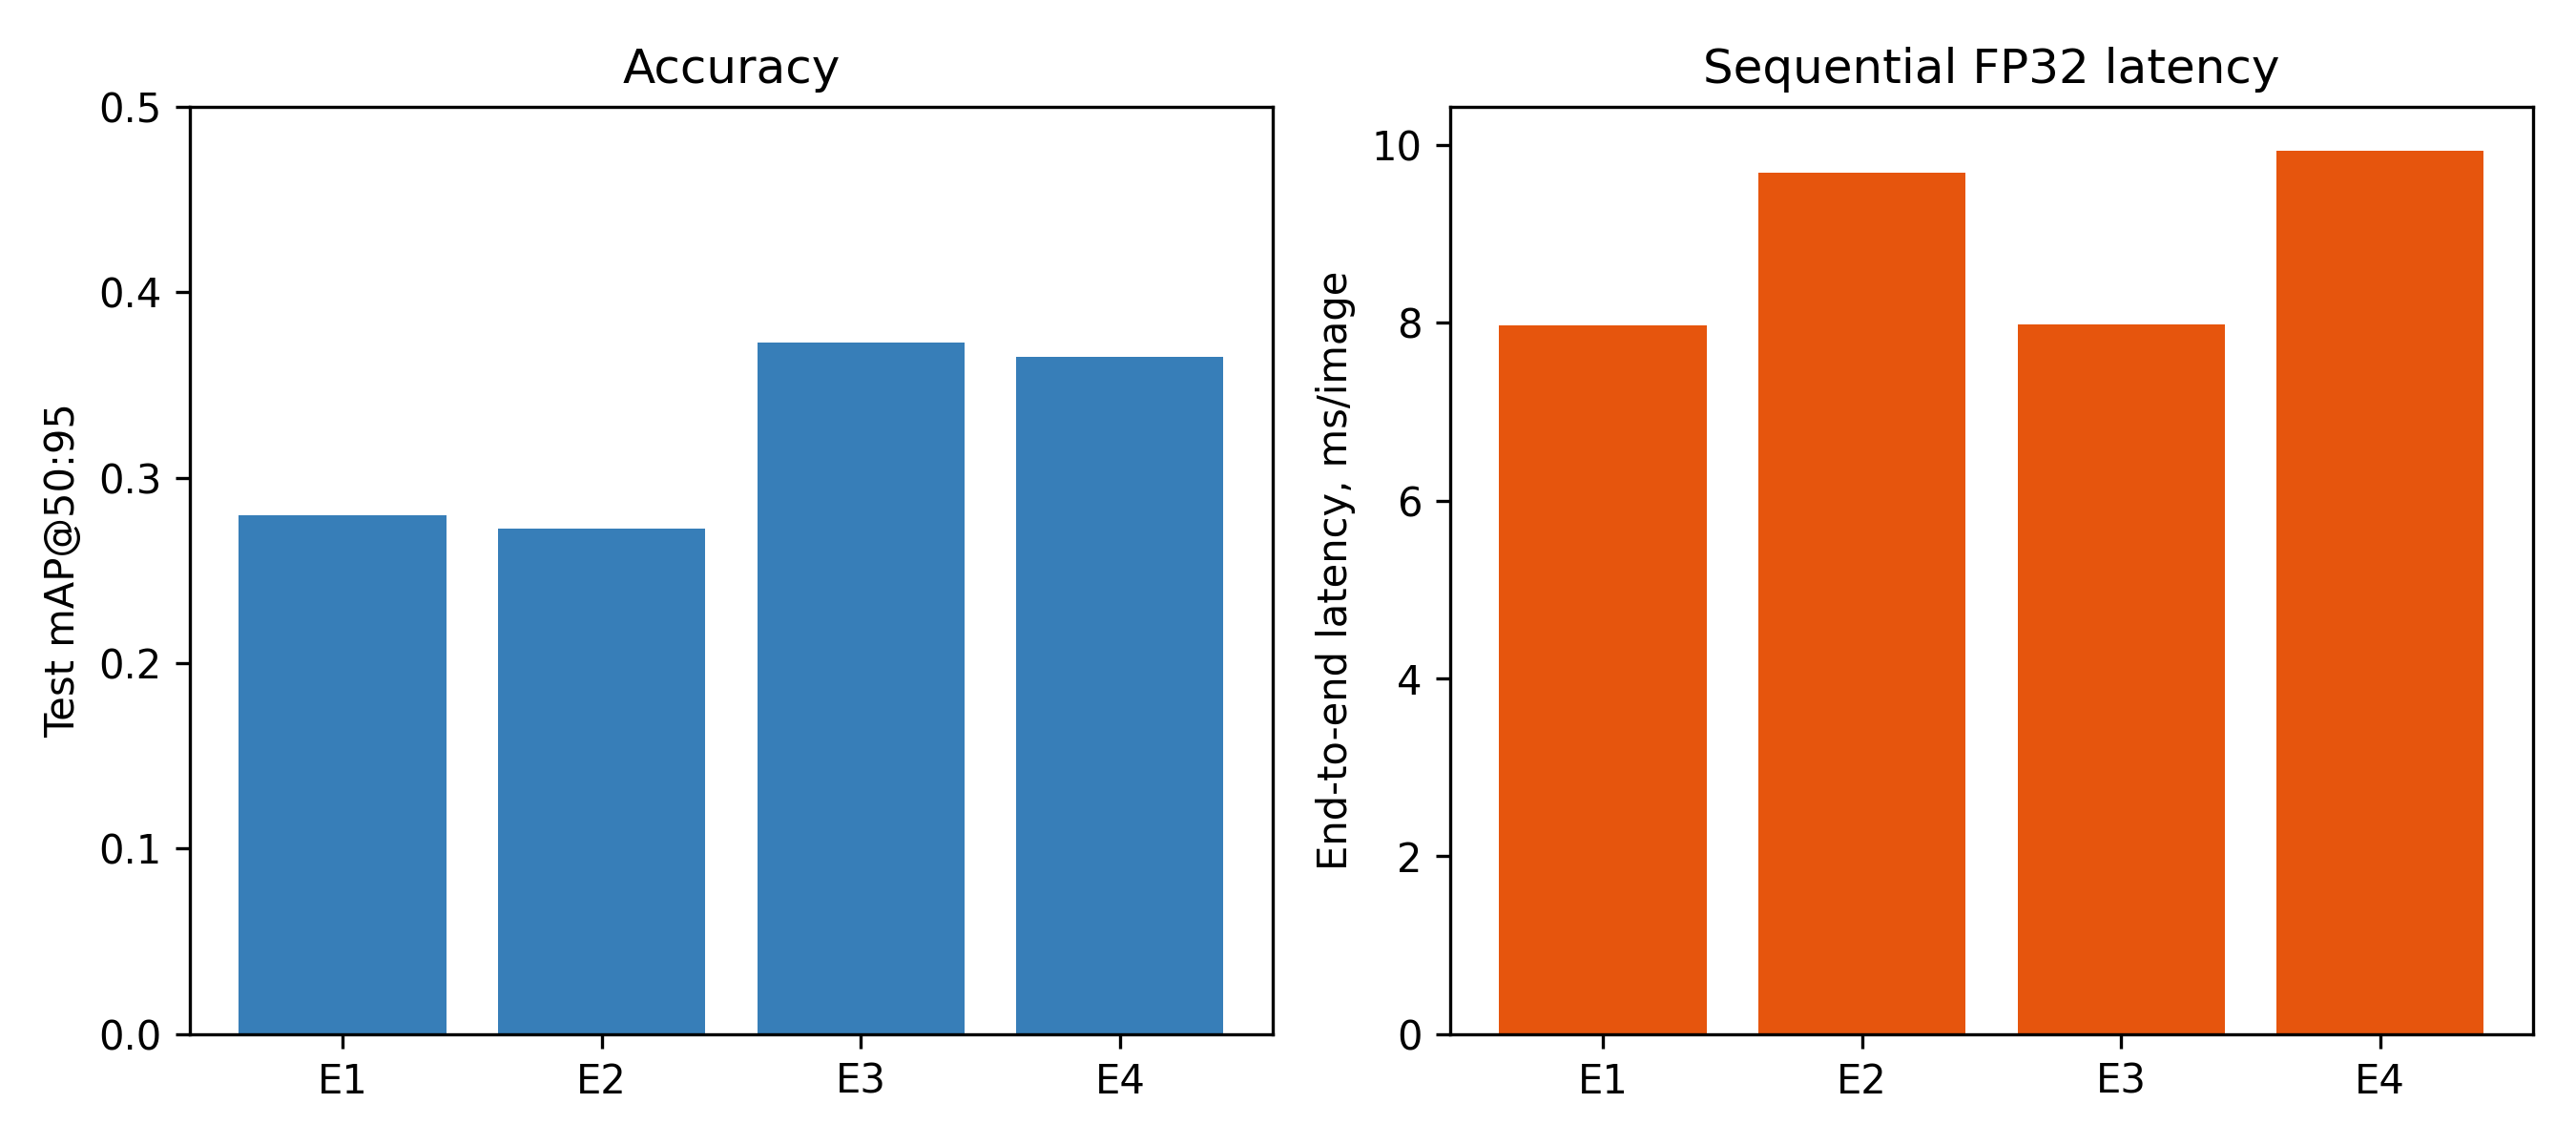
\includegraphics[width=\columnwidth]{figures/fig_7_quality_speed.png}
  \caption{Качество Test ($mAP@50{:}95$) и средняя E2E-задержка E1--E4.}
  \label{fig:tradeoff}
\end{figure}

Абсолютные значения задержки получены при повторении измерений \emph{одного} тестового изображения. Расчётная частота кадров как $1000/\overline t$ (при $\overline t$ в мс) не является независимым измерением пропускной способности и не должна обобщаться на производственную среду.

\subsection{Ограничения исследования}
Эксперименты проведены на одном разбиении NEU-DET при $\mathrm{seed}=42$. Повторные запуски с другими случайными начальными состояниями и статистическая проверка различий не выполнялись. Дополнительным ограничением являются изображения $200\times200$ пикселей и визуально похожие текстуры: хотя точные межвыборочные дубликаты отсутствуют, полную независимость внешнего вида объектов это не доказывает. Проверка на других производственных данных и на нескольких аппаратных платформах не проводилась. Следовательно, полученные результаты характеризуют контролируемое сравнение моделей, но не подтверждают готовность системы к внедрению.

\balance
\section{Заключение}
Проведено сравнение YOLOv8n и YOLO11n в четырёх конфигурациях при обнаружении шести типов дефектов стальной поверхности на NEU-DET. Применение умеренных аугментаций сопровождалось повышением $mAP@50{:}95$ для обеих архитектур на 9,33 и 9,27 п.п. соответственно. Наилучшие показатели в данном эксперименте получены для YOLOv8n с аугментациями: $mAP@50{:}95=37{,}29\%$, фиксированный $F_1=67{,}25\%$ при средней E2E-задержке 7,98 мс. Поклассовый анализ выявил трудности распознавания \textit{crazing} и \textit{rolled-in scale}, а оценка малых объектов показала различия между конфигурациями по числу пропусков. В дальнейшем целесообразны повторные запуски, внешняя проверка на независимых промышленных данных и отдельное изучение слабовыраженных и малых дефектов.

% Библиографические сведения проверены по DOI/официальным публикациям.
\begin{thebibliography}{15}
\bibitem{ibrahim2024} Ibrahim A.~A.~M.~S., Tapamo J.-R. A Survey of Vision-Based Methods for Surface Defects' Detection and Classification in Steel Products // \textit{Informatics}. 2024. Vol.~11, no.~2. Art.~25. DOI:~\href{https://doi.org/10.3390/informatics11020025}{10.3390/informatics11020025}.
\bibitem{chazhoor2024} Chazhoor A.~A.~P., Ho E.~S.~L., Gao B., Woo W.~L. A Review and Benchmark on State-of-the-Art Steel Defects Detection // \textit{SN Computer Science}. 2024. Vol.~5. Art.~114. DOI:~\href{https://doi.org/10.1007/s42979-023-02436-2}{10.1007/s42979-023-02436-2}.
\bibitem{redmon2016} Redmon J., Divvala S., Girshick R., Farhadi A. You Only Look Once: Unified, Real-Time Object Detection // \textit{CVPR}. 2016. P.~779--788. DOI:~\href{https://doi.org/10.1109/CVPR.2016.91}{10.1109/CVPR.2016.91}.
\bibitem{jocher2023} Jocher G., Chaurasia A., Qiu J. Ultralytics YOLOv8. Версия 8.0.0 [Программное обеспечение]. 2023. URL:~\url{https://docs.ultralytics.com/models/yolov8/}.
\bibitem{jocher2024} Jocher G., Qiu J. Ultralytics YOLO11. Версия 11.0.0 [Программное обеспечение]. 2024. URL:~\url{https://docs.ultralytics.com/models/yolo11/}.
\bibitem{liu2024} Liu L.-J., Zhang Y., Karimi H.~R. Resilient machine learning for steel surface defect detection based on lightweight convolution // \textit{Int. J. Adv. Manuf. Technol.} 2024. Vol.~134. P.~4639--4650. DOI:~\href{https://doi.org/10.1007/s00170-024-14403-z}{10.1007/s00170-024-14403-z}.
\bibitem{ni2025} Ni Y., Wu Q., Zhang X. FMR-YOLO: An improved YOLOv8 algorithm for steel surface defect detection // \textit{IET Image Processing}. 2025. Vol.~19. Art.~e70009. DOI:~\href{https://doi.org/10.1049/ipr2.70009}{10.1049/ipr2.70009}.
\bibitem{li2026} Li J., Yang Y., Geng R., Chang Y., Jiang Y., Wu K., Lu J. YOLOv11-LLR: An Enhanced Framework for Steel Surface Defect Detection in Industrial Settings // \textit{Applied Sciences}. 2026. Vol.~16, no.~10. Art.~4609. DOI:~\href{https://doi.org/10.3390/app16104609}{10.3390/app16104609}.
\bibitem{gaskarov2020} Гаскаров Р.~Д., Бирюков А.~М., Никонов А.~Ф., Агниашвили Д.~В., Хайрисламов Д.~А. Определение дефектов на стальных листах с использованием сверточных нейронных сетей // \textit{Электронные библиотеки}. 2020. Т.~23, №~6. С.~1155--1171. DOI:~\href{https://doi.org/10.26907/1562-5419-2020-23-6-1155-1171}{10.26907/1562-5419-2020-23-6-1155-1171}.
\bibitem{andriyanov2023} Андриянов Н.~А., Волненко А.~А., Дементьев В.~Е. Мониторинг состояния металлических изделий на основе систем компьютерного зрения // \textit{Нейрокомпьютеры: разработка, применение}. 2023. Т.~25, №~5. С.~50--57. DOI:~\href{https://doi.org/10.18127/j19998554-202305-07}{10.18127/j19998554-202305-07}.
\bibitem{vasiliev2024} Васильев М.~Е., Коськин А.~В., Шалимов А.~С. Автоматизация обнаружения дефектов поверхностей изделий на основе сверточных нейронных сетей // \textit{Вестник компьютерных и информационных технологий}. 2024. Т.~21, №~3. С.~30--36. DOI:~\href{https://doi.org/10.14489/vkit.2024.03.pp.030-036}{10.14489/vkit.2024.03.pp.030-036}.
\bibitem{shorten2019} Shorten C., Khoshgoftaar T.~M. A survey on Image Data Augmentation for Deep Learning // \textit{Journal of Big Data}. 2019. Vol.~6. Art.~60. DOI:~\href{https://doi.org/10.1186/s40537-019-0197-0}{10.1186/s40537-019-0197-0}.
\bibitem{song2013} Song K., Yan Y. A noise robust method based on completed local binary patterns for hot-rolled steel strip surface defects // \textit{Applied Surface Science}. 2013. Vol.~285. P.~858--864. DOI:~\href{https://doi.org/10.1016/j.apsusc.2013.09.002}{10.1016/j.apsusc.2013.09.002}.
\bibitem{he2020} He Y., Song K., Meng Q., Yan Y. An End-to-End Steel Surface Defect Detection Approach via Fusing Multiple Hierarchical Features // \textit{IEEE Trans. Instrum. Meas.} 2020. Vol.~69, no.~4. P.~1493--1504. DOI:~\href{https://doi.org/10.1109/TIM.2019.2915404}{10.1109/TIM.2019.2915404}.
\bibitem{lin2014} Lin T.-Y., Maire M., Belongie S., Hays J., Perona P., Ramanan D., Dollár P., Zitnick C.~L. Microsoft COCO: Common Objects in Context // \textit{ECCV}. 2014. P.~740--755. DOI:~\href{https://doi.org/10.1007/978-3-319-10602-1_48}{10.1007/978-3-319-10602-1\_48}.
\end{thebibliography}
\end{document}
